\section*{Problem No.3} \label{sec:prob3}

\paragraph{Part (A):} We can show the bounds of the growth factor on a square matrix $n \times n$ by considering the square matrix of the following structure:
\begin{enumerate}
\item The diagonal entries are ones
\item All the sub-diagonal entries are -1
\item All the super-diagonal entries are zeros expect the last column entries are ones.
\end{enumerate} 

We can should that when Gaussian elimiation with partial pivot is applied on matrix of such structure, it turns out that it is a systemic process of doubling the last column entries. For example, for $A \in \mathbb{R}^{5\times 5}$

\[A =
\left| 
\begin{array}{cc cc c}
 1 &  0 &  0 &  0 & 1  \\
-1 &  1 &  0 &  0 & 1  \\
-1 & -1 &  1 &  0 & 1  \\
-1 & -1 & -1 &  1 & 1  \\
-1 & -1 & -1 & -1 & 1  \\
\end{array} 
\right|
\] 
The first step of the elimination sum the first row with all other rows. The results would be such that the final column (except first entry) is doubled as shown in $U_{1}$. Next step will be summing the second row with all subsequent rows which double all entries of the last column (except first two) again as shown in $U_{2}$
\[U_{1} =
\left| 
\begin{array}{cc cc c}
1 &  0 &  0 &  0 & 1  \\
0 &  1 &  0 &  0 & 2  \\
0 & -1 &  1 &  0 & 2  \\
0 & -1 & -1 &  1 & 2  \\
0 & -1 & -1 & -1 & 2  \\
\end{array} 
\right| \quad \quad \quad \quad
U_{2} =
\left| 
\begin{array}{cc cc c}
1 &  0 &  0 &  0 & 1  \\
0 &  1 &  0 &  0 & 2  \\
0 &  0 &  1 &  0 & 4  \\
0 &  0 & -1 &  1 & 4  \\
0 &  0 & -1 & -1 & 4  \\
\end{array} 
\right|
\] 

The process keeps repeating with doubling the entries of the last column $n-$steps. For the given $A$, the matrix $U$ is:
\[
U =
\left| 
\begin{array}{cc cc c}
1 &  0 &  0 &  0 & 1  \\
0 &  1 &  0 &  0 & 2  \\
0 &  0 &  1 &  0 & 4  \\
0 &  0 &  0 &  1 & 6  \\
0 &  0 &  0 &  0 & 8  \\
\end{array} 
\right|
\] 
Thus, the growth factor is 
\[
\rho = \frac{max_{i,j}|u_{i,j}|}{max_{i,j}|a_{i,j}|} = 8 = 2^{m-1}
\]

With matrices of similar structure, the growth factor will be always  $2^{m-1}$. 

\paragraph{Part (B) \& (C):}
Figure \ref{fig:3b} shows relation between the growth factor and matrix sizes of random entries sampled uniformly from $[-1,1]$ without (left) and with (right) log-log scaling. Measuring the slope of the line fit on log-log scale date, the growth factor appears equal to $n^{0.52}$. Extrapolating this result to matrix of size $10^{6} \times 10^{6}$, the growth rate would be $10^{3}$.
 
\begin{figure}[tbh]
 \centering  
   {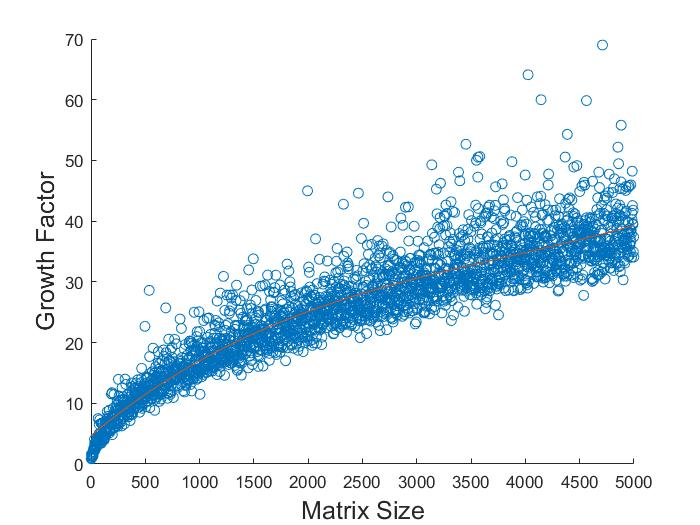
\includegraphics[width=0.48\linewidth]{code/prob3_nolog.jpg}}   
   {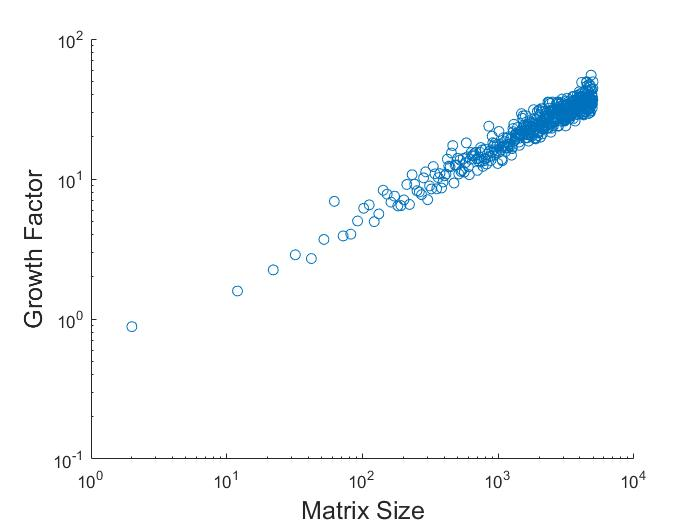
\includegraphics[width=0.48\linewidth]{code/prob3_log.jpg}}
  \caption{Scatter plots for the growth factor with matrix size without log-scale (left) and on log-log scale (right) for matrices of different sizes along with the polynomial being fit for interpolation.}
   \label{fig:3b}
\end{figure} 